\chapter{What Are We Trying to Explain?}
\label{ch:scientific-problem}

\textit{The empirical problem is not only that cortical spike trains are irregular. It is that repeated presentations of the same condition produce variable spike counts, slow shared fluctuations, and stimulus-dependent reductions in variability. Clustered spiking networks are interesting because they can keep fast irregular spiking while adding a slower latent state: which clusters are active.}

% ============================================================
\section{Trial-to-trial neural variability}
\label{sec:trial-to-trial-neural-variability}
% ============================================================

A trial is a repeated attempt to observe the same neural system under nominally the same condition. In a sensory experiment the condition might be one stimulus. In a simulation it might be the same external input, same parameters, and different random seeds. Trial-to-trial variability means that the measured spike trains are not identical across repetitions.

For neuron $i$ on trial $q$, write the spike train as
%
\begin{equation}
  s_i^{(q)}(t)=\sum_m \delta(t-t_{i,m}^{(q)}),
  \label{eq:trial-spike-train}
\end{equation}
%
where $t_{i,m}^{(q)}$ is the time of the $m$th spike on that trial. The spike count in a window $W=[t_0,t_0+T]$ is
%
\begin{equation}
  N_i^{(q)}(W)
  =
  \int_{t_0}^{t_0+T} s_i^{(q)}(t)\,\dd t .
  \label{eq:trial-spike-count}
\end{equation}
%
The integral counts impulses. It discards exact spike times inside the window and keeps one scalar: how many spikes occurred.

Across $R$ repeated trials, the empirical mean and variance are
%
\begin{equation}
  \widehat\mu_i(W)
  =
  \frac{1}{R}\sum_{q=1}^R N_i^{(q)}(W),
  \qquad
  \widehat\sigma_i^2(W)
  =
  \frac{1}{R-1}\sum_{q=1}^R
  \left(N_i^{(q)}(W)-\widehat\mu_i(W)\right)^2.
  \label{eq:trial-count-mean-variance}
\end{equation}
%
$\widehat\mu_i$ measures response magnitude in that window. $\widehat\sigma_i^2$ measures reliability. If $\widehat\sigma_i^2$ is large, the same nominal condition can lead to very different observed responses.

The word ``same'' hides an important modeling choice. Trials may share the same stimulus, but they do not necessarily share the same internal network state. A clustered network can begin one trial with different clusters near up-states than another trial. Then the variability is not only spike-generation noise; it is variability in the latent state from which the trial begins.

The first practical computation is therefore simple: choose a window $W$, compute $N_i^{(q)}(W)$ across trials, and ask whether the variance is consistent with independent spiking at a fixed rate or whether it requires slower hidden state fluctuations.

% ============================================================
\section{Fano factor, CV, and super-Poisson spiking}
\label{sec:fano-cv-super-poisson-spiking}
% ============================================================

Two statistics appear repeatedly in this project. The Fano factor measures count variability. The coefficient of variation measures interval irregularity.

\begin{keyequation}[Spike-Count Fano Factor]
\begin{equation}
  F_i(T)
  =
  \frac{\Var[N_i(T)]}{\E[N_i(T)]}.
  \label{eq:chapter1-fano-factor}
\end{equation}
\tcblower
$N_i(T)$ is the spike count in a window of duration $T$; the numerator is trial-to-trial count variance; the denominator is the mean count. A homogeneous Poisson process has $F_i(T)=1$.
\end{keyequation}

\noindent If $F_i(T)<1$, counts are more regular than Poisson. If $F_i(T)>1$, counts are overdispersed or \emph{super-Poisson}. Super-Poisson variability is common when the firing rate itself fluctuates across trials or over slow time scales.

The coefficient of variation of interspike intervals is
%
\begin{equation}
  \mathrm{CV}_i
  =
  \frac{\sqrt{\Var[T_i^m]}}{\E[T_i^m]},
  \qquad
  T_i^m=t_{i,m+1}-t_{i,m}.
  \label{eq:chapter1-cv}
\end{equation}
%
The numerator is the standard deviation of intervals. The denominator is the mean interval, so CV is dimensionless. Nearly periodic spiking has $\mathrm{CV}\ll 1$; Poisson-like irregular spiking has $\mathrm{CV}\approx 1$; bursting or long silent gaps can give $\mathrm{CV}>1$.

Fano factor and CV are related but not interchangeable. CV asks whether adjacent spikes are regular. Fano factor asks whether counts are reliable in a chosen window. A neuron can have $\mathrm{CV}\approx 1$ inside each network state while having $F(T)\gg 1$ over long windows because the state itself switches slowly.

A useful baseline is a doubly stochastic or Cox-process count model. Let $\Lambda_T$ be the integrated rate in the counting window. Conditional on $\Lambda_T$, assume the spike count is Poisson:
%
\begin{equation}
  N_T\mid \Lambda_T \sim \operatorname{Poisson}(\Lambda_T).
  \label{eq:cox-count-model}
\end{equation}
%
Then the law of total variance gives
%
\begin{keyequation}[Fano Factor with Slow Rate Fluctuations]
\begin{equation}
  \E[N_T]=\E[\Lambda_T],
  \qquad
  \Var[N_T]=\E[\Lambda_T]+\Var[\Lambda_T],
  \qquad
  F(T)=1+\frac{\Var[\Lambda_T]}{\E[\Lambda_T]}.
  \label{eq:fano-total-variance}
\end{equation}
\tcblower
The Poisson term $\E[\Lambda_T]$ is fast counting noise. The extra term $\Var[\Lambda_T]$ is slow rate variability across trials or windows.
\end{keyequation}

\noindent This equation is the core intuition for super-Poisson counts. If the integrated rate changes from trial to trial, the Fano factor rises above one even if spiking is conditionally Poisson within each trial.

The next computation is to plot $F(T)$ as a function of window duration $T$ and compare it with CV. A large-window Fano factor that grows while CV stays near one points toward slow latent fluctuations rather than simply more irregular spike generation.

% ============================================================
\section{Slow fluctuations vs fast irregular spiking}
\label{sec:slow-fluctuations-fast-irregular-spiking}
% ============================================================

Fast irregular spiking and slow fluctuations live at different levels. Fast irregularity concerns spike timing around the current instantaneous intensity. Slow fluctuation concerns changes in the intensity or latent network state itself.

One compact decomposition is
%
\begin{equation}
  s_i(t)
  =
  \lambda_i(t)
  +
  \varepsilon_i(t),
  \label{eq:spike-train-rate-noise-decomposition}
\end{equation}
%
where $s_i(t)$ is the spike train, $\lambda_i(t)$ is a conditional intensity or smoothed rate, and $\varepsilon_i(t)$ is the fast point-process innovation. This is not a deterministic equality between ordinary functions; it is a statistical decomposition. The intensity carries predictable structure given the current state. The innovation is the remaining spike-time randomness.

If $\lambda_i(t)$ is nearly constant across trials, count variability mainly reflects point-process noise. If $\lambda_i(t)$ changes slowly because the network wanders among cluster states, spike counts inherit that slow variability. In that case, long windows contain two contributions:
%
\begin{equation}
  N_i(T)
  =
  \int_0^T \lambda_i(t)\,\dd t
  +
  \int_0^T \varepsilon_i(t)\,\dd t .
  \label{eq:count-slow-fast-contributions}
\end{equation}
%
The first term is the integrated latent drive. The second term is the accumulated fast spiking innovation. Increasing the counting window averages some fast noise, but it can amplify the effect of slow changes in $\lambda_i(t)$.

Autocorrelation makes the same distinction. For a smoothed rate $r_i(t)$,
%
\begin{equation}
  \rho_i(\tau)
  =
  \frac{\E[(r_i(t)-\mu_i)(r_i(t+\tau)-\mu_i)]}{\Var[r_i(t)]}.
  \label{eq:chapter1-autocorrelation}
\end{equation}
%
Fast irregular spiking produces short autocorrelation. Cluster-state switching can produce a long tail because the present cluster state predicts the future for the duration of a dwell time.

For the rotation, the practical question is not whether the raster looks irregular. It will. The question is whether the irregularity contains a slow component that can be represented by cluster variables such as $m_k(t)$, $r_k(t)$, or the number of active clusters $n_{\mathrm{act}}(t)$.

% ============================================================
\section{Spontaneous vs stimulus-evoked variability}
\label{sec:spontaneous-vs-stimulus-evoked-variability}
% ============================================================

Spontaneous activity is measured without a controlled time-varying stimulus. Evoked activity is measured after aligning trials to a stimulus or task event. The same statistic can mean different things in the two settings.

In spontaneous activity, one often estimates variability from windows sampled across a long recording:
%
\begin{equation}
  N_i^{(b)}(T)
  =
  \int_{bT}^{(b+1)T}s_i(t)\,\dd t ,
  \label{eq:spontaneous-window-counts}
\end{equation}
%
where $b$ indexes non-overlapping windows. This is useful only if the process is approximately stationary over the analyzed period. Slow drift, adaptation, or task-state contamination can inflate the estimated variance.

In evoked activity, the mean response is time dependent. The peristimulus time histogram estimates
%
\begin{equation}
  \widehat r_i(t)
  =
  \frac{1}{R}\sum_{q=1}^R
  (\kappa*s_i^{(q)})(t),
  \label{eq:psth-estimator}
\end{equation}
%
where $\kappa$ is a smoothing kernel. Trial-to-trial variability should then be computed around the stimulus-locked mean, not around a single stationary baseline.

A useful residual count is
%
\begin{equation}
  \Delta N_i^{(q)}(W)
  =
  N_i^{(q)}(W)
  -
  \E[N_i(W)\mid \text{stimulus condition}],
  \label{eq:evoked-residual-count}
\end{equation}
%
which measures how trial $q$ differs from the condition average. If residual variability drops after stimulus onset, the stimulus has made the response more reliable in a way that is not explained solely by the mean response profile.

In clustered networks, spontaneous and evoked variability differ because the stimulus changes the distribution over cluster states. Spontaneous activity may explore many active-cluster configurations. A stimulus may favor a smaller subset. The mean rate can rise while the latent-state variance falls.

The next computation is to estimate variability before and after stimulus onset with mean matching whenever possible. A reduced Fano factor after stimulus onset is most informative when it survives controls for changes in mean count.

% ============================================================
\section{Variability quenching after stimulus onset}
\label{sec:variability-quenching-after-stimulus-onset}
% ============================================================

Variability quenching means that neural responses become less variable after stimulus onset. The word should not be read as ``spikes become regular.'' It often means that a slow shared component of variability is reduced.

\begin{aside}[Citation TODO]
Add empirical citations for stimulus-onset reductions in spike-count variability and Fano factor after the bibliography pass. The claims in this section should be tied to primary experimental reports or an appropriate review before final release.
\end{aside}

Using the integrated-intensity decomposition, a pre/post comparison can be written schematically as
%
\begin{equation}
  F_{\mathrm{pre}}(T)
  =
  1+
  \frac{\Var[\Lambda_T^{\mathrm{pre}}]}{\E[\Lambda_T^{\mathrm{pre}}]},
  \qquad
  F_{\mathrm{post}}(T)
  =
  1+
  \frac{\Var[\Lambda_T^{\mathrm{post}}]}{\E[\Lambda_T^{\mathrm{post}}]} .
  \label{eq:pre-post-fano-quenching}
\end{equation}
%
The Fano factor drops when the ratio $\Var[\Lambda_T]/\E[\Lambda_T]$ drops. That can happen even if the fast point-process part remains Poisson-like and even if the mean firing rate increases.

\begin{figure}[h]
\centering
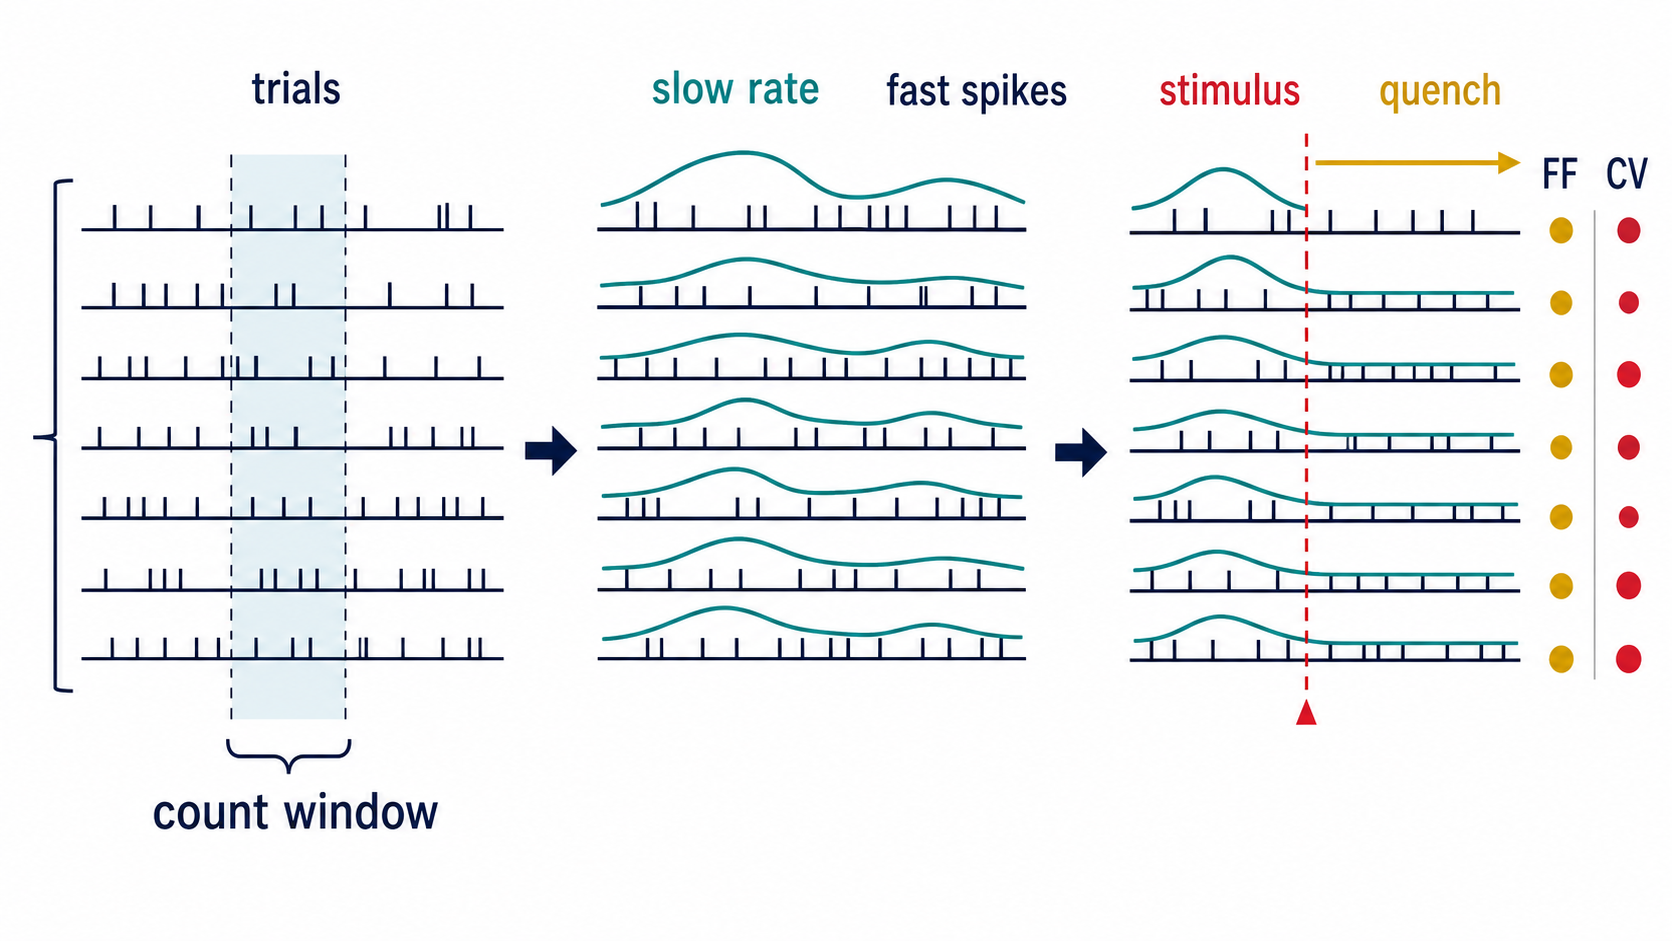
\includegraphics[width=0.95\textwidth]{figures/meso-variability-decomposition.png}
\caption{Trial-to-trial variability has more than one source. Fast irregular spike timing affects CV-like measures, while slow trial-level rate envelopes inflate spike-count variability and Fano factor. A stimulus can reduce the slow envelope, producing variability quenching even when spikes remain irregular.}
\label{fig:variability-decomposition}
\end{figure}

Clustered networks give a concrete latent-state version of this idea. Let $Z$ denote the cluster state during a window: for example, which clusters are active. Conditional on $Z$, suppose a neuron has mean count $\mu_Z$. Across trials,
%
\begin{equation}
  \Var[N_T]
  =
  \E[\Var[N_T\mid Z]]
  +
  \Var[\E[N_T\mid Z]]
  =
  \E[\mu_Z]
  +
  \Var[\mu_Z]
  \label{eq:state-mixture-fano}
\end{equation}
%
under a conditional Poisson approximation. The first term is within-state spiking variability. The second term is across-state variability. A stimulus quenches variability if it reduces the spread of $\mu_Z$ by concentrating probability on fewer states or by making the allowed states more similar.

This equation also warns against a common mistake. A lower post-stimulus Fano factor does not prove that each neuron became less noisy. It may mean that the network was pushed into a more reproducible region of state space.

% ============================================================
\section{Why clustered networks are a candidate mechanism}
\label{sec:why-clustered-networks-candidate-mechanism}
% ============================================================

A clustered network supplies a mechanistic latent variable. Instead of assuming an abstract fluctuating gain, it proposes that groups of neurons enter and leave high-activity states.

Let $m_k(t)\in\{0,1\}$ be an idealized activity indicator for cluster $k$: $m_k=1$ when the cluster is in an up-state and $m_k=0$ when it is in a down-state. A simple observation model for neuron $i$ is
%
\begin{equation}
  \lambda_i(t)
  =
  \lambda_{i,0}
  +
  \sum_{k=1}^K b_{ik}m_k(t),
  \label{eq:cluster-latent-rate-model}
\end{equation}
%
where $\lambda_{i,0}$ is baseline intensity and $b_{ik}$ measures how strongly active cluster $k$ changes neuron $i$'s firing intensity. For neurons inside cluster $k$, $b_{ik}$ is usually positive and large. For neurons in competing clusters, it may be smaller or effectively negative after inhibition is included.

This model is intentionally simple, but it gives the right measurement predictions:
%
\begin{enumerate}[leftmargin=*]
  \item If $m_k(t)$ changes slowly, spike counts have slow variability and long autocorrelation.
  \item If only a few clusters are active at a time, neurons in the same active cluster share variability.
  \item If a stimulus biases the network toward a smaller set of cluster states, Fano factors can decrease after stimulus onset.
  \item If spikes remain irregular inside each state, CV can stay near one while count variability changes.
\end{enumerate}

The mechanism is attractive because it bridges scales. At the microscopic level, recurrent excitatory synapses inside a cluster help sustain activity. At the mesoscopic level, the cluster activity variable is a state coordinate. At the measurement level, slow changes in that coordinate appear as trial-to-trial variability.

The computation to do next is to extract cluster-state variables from a simulation: smoothed cluster rates $r_k(t)$, binary indicators $m_k(t)$, active-cluster count $n_{\mathrm{act}}(t)$, cluster lifetimes, and autocorrelations. These are the observables a mesoscopic theory must reproduce.

% ============================================================
\section{The core rotation question: microscopic simulation or mesoscopic theory?}
\label{sec:core-rotation-question}
% ============================================================

A microscopic simulation can answer whether a particular network switches among cluster states. It cannot by itself explain which parts of the result are robust, which depend on finite size, and which should persist under a change of architecture.

A mesoscopic theory tries to keep the variables that matter for the switching:
%
\begin{equation}
  \vec r(t)
  =
  (r_1(t),\ldots,r_K(t)),
  \qquad
  n_{\mathrm{act}}(t)=\sum_{k=1}^K \mathbf{1}\{r_k(t)>\theta_{\mathrm{up}}\}.
  \label{eq:chapter1-mesoscopic-cluster-variables}
\end{equation}
%
$\vec r(t)$ records cluster rates. The thresholded count $n_{\mathrm{act}}$ records how many clusters are active. Varying $\theta_{\mathrm{up}}$ changes the detection rule, so the rule must be reported and tested for robustness.

The central theoretical fork is
%
\begin{equation}
  \text{stable attractors plus finite-size noise}
  \qquad
  \text{versus}
  \qquad
  \text{deterministic mesoscopic irregularity}.
  \label{eq:chapter1-theory-fork}
\end{equation}
%
In the first picture, deterministic dynamics create stable or metastable cluster states, and finite population fluctuations kick the network between them. In the second picture, the reduced population dynamics may be irregular even without finite-size noise.

A minimal stochastic mesoscopic equation writes this distinction explicitly:
%
\begin{equation}
  \dd \vec r
  =
  \vec f(\vec r;\theta)\,\dd t
  +
  \frac{1}{\sqrt{N_c}}\,
  \mat G(\vec r;\theta)\,\dd \vec W_t .
  \label{eq:chapter1-mesoscopic-sde}
\end{equation}
%
$\vec f$ is the deterministic drift of the cluster rates. $\theta$ collects coupling strengths, external input, and time constants. $\mat G$ sets the covariance of finite-size fluctuations. $N_c$ is a representative cluster size. If switching is finite-size driven, increasing $N_c$ while holding the deterministic drift fixed should reduce switching. If switching persists in the large-size limit, the deterministic drift or quenched disorder must be doing more of the work.

The rotation should therefore produce more than a reproduction raster. It should produce a comparison between microscopic simulations and mesoscopic predictions: fixed points, stability, dwell times, finite-size scaling, and stimulus-induced changes in state occupancy.

\begin{chaptersummary}

\begin{center}
\renewcommand{\arraystretch}{1.55}
\begin{tabularx}{\textwidth}{@{}l X X@{}}
  \toprule
  \textbf{Concept} & \textbf{Equation} & \textbf{What to notice} \\
  \midrule
  Spike count &
  $N_i(W)=\int_W s_i(t)\,\dd t$ &
  Counts define trial-to-trial response variability in a chosen window \\
  Fano factor &
  $F(T)=\Var[N_T]/\E[N_T]$ &
  Overdispersion means more variability than fixed-rate Poisson spiking \\
  ISI CV &
  $\mathrm{CV}=\sqrt{\Var[T_m]}/\E[T_m]$ &
  Interval irregularity is distinct from long-window count variability \\
  Slow-rate contribution &
  $F=1+\Var[\Lambda_T]/\E[\Lambda_T]$ &
  Fluctuating integrated rate inflates counts above Poisson \\
  State-mixture contribution &
  $\Var[N]=\E[\Var(N\mid Z)]+\Var[\E(N\mid Z)]$ &
  Latent cluster states create extra trial-to-trial variability \\
  Cluster latent rate &
  $\lambda_i=\lambda_{i,0}+\sum_k b_{ik}m_k$ &
  Active clusters turn network state into measurable firing-rate variability \\
  Mesoscopic fork &
  $\dd\vec r=\vec f\,\dd t+N_c^{-1/2}\mat G\,\dd\vec W_t$ &
  Scaling with cluster size tests finite-size switching \\
  \bottomrule
\end{tabularx}
\end{center}

\end{chaptersummary}

\begin{conceptquestions}
  \item Why is trial-to-trial variability not fully described by the visual irregularity of a single-trial raster?
  \item A neuron has $\mathrm{CV}\approx 1$ but $F(1\,\mathrm{s})=3$. What mechanism could make these two facts compatible?
  \item Use the law of total variance to explain why a fluctuating integrated intensity $\Lambda_T$ raises the Fano factor above one.
  \item What does variability quenching mean if individual spikes remain irregular after stimulus onset?
  \item In the state-mixture model, what experimental or simulation observation would indicate that $\Var[\E(N\mid Z)]$ decreased after stimulus onset?
  \item Why are cluster rates $r_k(t)$ better candidate mesoscopic variables than the global excitatory rate when studying clustered networks?
  \item What finite-size scaling result would support the hypothesis that metastable switching is noise-driven escape among stable cluster states?
\end{conceptquestions}

\clearpage
